\section {Tkinter}

\subsection{Definisi}
\cite{lundh1999introduction} Modul Tkinter atau Tk interface adalah Python interface standar ke toolkit Tk GUI dari Scriptics yang sebelumnya dikembangkan oleh Sun Labs. Baik Tk dan Tkinter tersedia di sebagian besar platform Unix, begitu juga pada sistem Windows dan Macintosh. Dimulai dengan rilis 8.0, Tk menawarkan tampilan dan nuansa asli pada semua platform. Tkinter terdiri dari sejumlah modul. Antarmuka Tk terletak di modul biner bernama _tkinter (ini tkinter di versi sebelumnya). Modul ini berisi antarmuka tingkat rendah ke Tk, dan tidak boleh digunakan langsung oleh pemrogram aplikasi. Ini biasanya adalah shared library (atau DLL), tetapi mungkin dalam beberapa kasus terhubung secara statis dengan penerjemah Python. Selain modul antarmuka Tk, Tkinter menyertakan sejumlah modul Python. Dua modul yang paling penting adalah modul Tkinter itu sendiri, dan modul yang disebut Tkconstants. Yang pertama secara otomatis mengimpor yang terakhir, jadi untuk menggunakan Tkinter, semua yang perlu Anda lakukan adalah mengimpor satu modul: 

\begin {verbatim}
	import Tkinter
\end {verbatim}
	
Atau, lebih sering:

\begin {verbatim} 
Form Tkinter import *
\end {verbatim}

\begin {table}
\centering
\begin {tabular}{|l|l|}
	\hline
	Widget & Deskripsi\\
	\hline
	Button & Tombol sederhana, digunakan untuk menjalankan perintah atau operasi lainnya\\
	\hline
	Canvas & Grafis terstruktur. Widget ini dapat digunakan untuk menggambar grafik dan plot, membuat editor grafis, dan mengimplementasikan widget khusus.\\
	\hline
	Checkbutton & Merupakan variabel yang dapat memiliki dua nilai berbeda. Mengklik tombol matikan antara nilai-nilai.\\
	\hline
	Entry & Bidang entri teks.\\
	\hline
	Frame & Widget penampung. Bingkai dapat memiliki batas dan latar belakang, dan digunakan untuk mengelompokkan widget lain saat membuat aplikasi atau tata letak dialog.\\
	\hline
	Label & Menampilkan teks atau gambar.\\
	\hline
	Listbox & Menampilkan daftar alternatif. Listbox dapat dikonfigurasi untuk mendapatkan radiobutton atau perilaku checklist.\\
	\hline
	Menu & Panel menu, Digunakan untuk mengimplementasikan menu pulldown dan popup.\\
	\hline
	Menubutton & Menubutton, Digunakan untuk mengimplementasikan menu pulldown.\\
	\hline
	Message & Tampilkan sebuah teks. Serupa dengan widget label, tetapi dapat secara otomatis membungkus teks ke lebar atau aspek rasio yang diberikan\\
	\hline
	Radiobutton & Mewakili satu nilai dari variabel yang dapat memiliki satu dari banyak nilai. Mengeklik tombol menyetel variabel ke nilai itu, dan menghapus semua tombol radio lain yang terkait dengan variabel yang sama.\\
	\hline
	Scale & Memungkinkan Anda menetapkan nilai numerik dengan menyeret "slider".\\
	\hline
	Scrollbar & Scrollbar standar untuk digunakan dengan kanvas, entri, listbox, dan teks widget.\\
	\hline
	Text & Format teks terformat. Memungkinkan Anda untuk menampilkan dan mengedit teks berbagai gaya dan atribut. Juga mendukung gambar yang disematkan dan windows.\\
	\hline
	Toplevel & Widget wadah ditampilkan sebagai jendela tingkat atas terpisah.\\
	
\end {tabular}
\end {table}
\subsection{Penggunaan Tkinter}
Tkinter biasa digunakan saat sebuah aplikasi python membutuhkan GUI dan harus menampilkan graphical interface untuk diberikan kepada pengguna. Contoh kode dari tkinter adalah sebagai berikut : 
\begin{verbatim}
from tkinter import Tk, Frame
class mengubahJudul(Frame):
    def __init__(self, parent):
        Frame.__init__(self, parent,)

        self.tampilan = parent

        self.initUI()

    def initUI(self):
        self.tampilan.title("ini judul nya")


if __name__ == '__main__':
    root = Tk()
    app = mengubahJudul(root)
    root.mainloop()
\end{verbatim}
Dari kode berikut, dapat menghasilkan GUI seperti berikut : 
	\begin{figure} [ht]
		\centerline{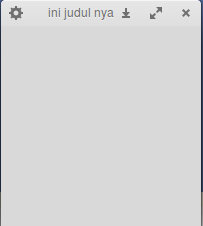
\includegraphics[width=1\textwidth]{figures/tkinterguiexample.png}}
		\caption{Hasil Program TKinter}
		\label{resultkinter}
	\end{figure}
Pada gambar \ref{resultkinter}, Koding menampilkan GUI dan menyetting judul dari program tersebut. Untuk kasus tertentu, dapat juga membuat seperti tombol, atau lainnya untuk kerja sistem tersendiri. Fungsi Tkinter dapat maksimal jika program memang besar. Tkinter juga seperti program GUI lainnya yaitu memiliki bagian seperti berikut : 
\begin{itemize}
	\item Frame : Sebagai tempat menyimpan isi dari tampilan - tampilan. Bisa dibilang layar dari GUI itu sendiri.	
	\item Header : Setting judul dari program.
	\item Footer : Biasa untuk mensetting credit atau pembuat aplikasi.
	\item Button : Sebagai tombol eksekusi fungsi yang telah disetting oleh programmer.
	\item Dialog : Sebagai popup dari program saat muncul sebuah notifikasi.
	\item Splash Screen : Tampilan pengenalan sebelum aplikasi telah berjalan.
	\item Background Manipulation : Memanipulasi atau mewarnai sebuah tampilan belakang dari sebuah frame.
\end{itemize}
\subsubsection{Kode aplikasi basic}
Ada contoh untuk membuat aplikasi simpel. Contoh ini menampilkan tampilan sederhana seperti frame saja. berikut adalah kodenya :
\begin{verbatim}
import tkinter
top = tkinter.Tk()
 
# kode widget simpan disini
 
top.mainloop()
\end{verbatim}
Untuk tampilan dari aplikasi bisa dilihat dengan mencobanya sendiri.
\subsection{Kesimpulan}
Tkinter adalah tool atau alat untuk membuat GUI Interface pada pemrograman python. Fungsi dari GUI pada tkinter cukup mirip dengan aplikasi berbasis GUI lainnya. TKinter tersedia dalam banyak platform atau sistem operasi seperti MacOS, Windows, ataupun Linux. TKinter dibuat untuk memudahkan dalam berinteraksi dengan bahasa python dengan pengguna.
